\chapter{第四格}

\begin{figure}[H]
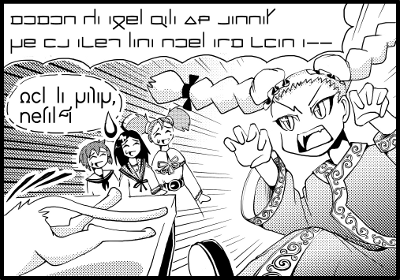
\includegraphics[width=0.5\textwidth]{ARKA/uni4.png}%或者height=\textheight
\end{figure}


\emoji{l_reia}
那个金毛丸子头就是``孩子气的Feel''哦。穿着叫做``teebe''的长袍。


\emoji{a_sm}
teebe也是Arna大学的制服,

テーベもアルナ大の制服で、像我这样的Raudura学院的学生经常穿。

普通科这么穿到时很少见……。


\emoji{l_nakx}
Feel虽说也是Arna的人,但就是有点怪。

她觉得自己是从神话时代转生过来的
\footnote{她以为自己是Kmiiir的转世.Kmiir则是Axet的一员,从恶魔手中拯救世界.}
。所以和占卜师Aria穿的是同样的teebe。

长得娇小(矮),所以有些烦恼、活泼得很,说话总是能这样那样地离题。

很会搞事情,但这样才有趣嘛。


\emoji{x_iks}
2333w  看那个脸 w

就像要把猫抓来吃了一样呢w

好像文字的设计也在这里变化了呢。好细啊。


\emoji{a_reps}
看,转写

\FiveStar 转写

feel: momon ca adel fala 85 sanna! re is axek lana noel atm xian a--


\emoji{x_demo}
额,首先momon是个啥。
    
\emoji{x_seernik}
……蛤?  [魔物]……?  啥啊。

----

momon

[魔物]momon(猫熊):第八十五天:利之空天

19:ridia/seren/mel : 源自叫声

[文化]

妖族。矮胖而像猫和熊。体型像大些的兔子。
它们有一个惹人爱的习惯,就是变化成人们饲养的宠物。会发出``momon''的奇怪声音。对主人忠实,很驯服。

----

\emoji{l_xanxa}
我快把这忘了,Arbazard还是异世界呢(-\_{}-; 也就是``剑与魔法的幻想''。

在我的时代已经绝迹了,曾经有100种魔物呢。

说``八十五天''是指momon是怪物里的第85号。

momon是很珍贵的魔物,不会伤害人类.就像宠物一样。

\emoji{l_ket}
我也想养一只momon啊。

为啥不来我家捏\~{}。


\emoji{x_nal}
モ○グリ啊,明白了。


\emoji{l_iks}
额……。


\emoji{x_niit}
ca是表示强调的形容词、像英语的the一样。

momon ca adel 就是``mmon・the・monsterー \FiveStar ''这样的感觉吧?

----

ca

[形容词]这。增加强调和限制意味,前置使用。

[形容词]表示后面的是固有名词。前置使用。

[名词]``*''号

17:制:古:ca(表示强调的形容词,有冠词性)

【用例】

varfant, ca freian 剑士Varfrant

----

\emoji{l_diina}

对,在同一格。","记号叫做``tsunk''、写不写都可以。

fala 85在上面也有提到、意思是85号的魔族。fala是表示序号的格词。


\emoji{x_loki}
sanna是表示确认的,总体来看``momon ca adel fala 85 sanna!''就是``你就是第八十五天的momon吧!''的意思呢。

哈啊,搁着Feel把猫当成魔物了。

确实、离谱的神話志向妹 (-ω-;

\begin{figure}[H]
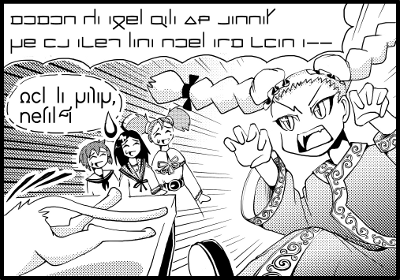
\includegraphics[width=0.5\textwidth]{ARKA/uni4.png}%或者height=\textheight
\end{figure}


\emoji{x_asex}
接下来是``re is axek lana noel atm xian a...''这句。

re在``命令・依頼・禁止''学过了,表示命令。

is是死生动词那一课的``死动词'',``关闭,停止''.


\emoji{l_deyu}
动词is的宾语是axek(変身)。

尽管日语的``変身を解く(解除变身)''里面要用``解く(解除)''作动词搭配、,Arka里直接写is就行了。

\emoji{x_niit}
因为宾语axek已经明确了,后面就不再带名词。

lana既有名词又有格词的用法、但这里确定是格词。表示``为了做''。

noel是我(私)、xian是你――指猫。

atm……``卖''。额、卖猫?


\emoji{l_reiv}
好像是  (-\_{}-;

haizen(报应啊)


\emoji{x_knoos}
最后的a是啥……。

唉、哎哎哎、a是什么意思啊!?


\emoji{a_sm}
在句末的话、应该是a(4)。只是整理语气,没有特别的意味。

----

a(4)

[文末纯词]"\~{}吗","\~{}嘛"\footnote{~だな、~か}。短的感叹。

古

[语法]

a系列用于自身。e系列用于听者。a系列对他人使用是男性的语气。
对于长辈和上级则失礼。即使是同级,如果不是非常要好,也会令人觉得草率。

----

\emoji{l_nax}
顺便一说,对他人说话还是用e比较合适。

只是,a还有额外的格词用法``为了~''。意思是``为了卖~''。

----

a

[格词]为~、为了~。与格。

[格词]向~对应的神祈祷时、不能用a,而应当用al。al karte就是沿袭古代祷词的用法.

13:制:al。为了区别于新的接续词al而改短了。

[语法]

动元音开头的单词用al。比如al an(向我)。

关系从句中只有格词残存的时候也用al。tu et ridia l'an fitat miik al(我给苹果的人是ridia)

【用例】

fit a lu. 给他。

fit al an. 给我。

----

\emoji{x_fron}
额……可是、a后面啥都没有了?卖的对象呢。


\emoji{l_niit}
这句话在这就截止了。

卖给谁就不清楚了、本来这里应该是买家的。

日语里台词的中间就有「(略」或者「(ry」的写法呢、只是不常用.


\emoji{x_loki}
啊,就是个「(略」。所以这里是只剩下格词 a 了吗。

那么整个句子、"re is axek lana noel atm xian a..."就是``现出原形!我要把你卖给......''这个感觉。

Feel把猫当成魔物变成的了。好奇怪的想法 (;´∀`)

不过,Aria,左上三个人一起说的是啥?。

\begin{figure}[H]
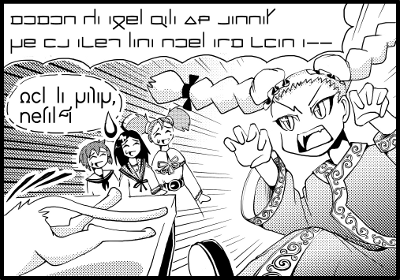
\includegraphics[width=0.5\textwidth]{ARKA/uni4.png}%或者height=\textheight
\end{figure}


\emoji{a_lo}
这是被Feel的举动整不会了。

最后的文字读作Alis,表示不安。转写写alis就可以了。

\FiveStar 转写

dil la rakar, netal (alis


\emoji{x_knoos}
dil是``阻碍,打断'',应该是动词、这就上动词了?

Arka 不是SVO语序吗?


\emoji{a_sm}
命令句里可以省略主语哦。


\emoji{x_nakx}
啊,是这,这么说前面确实有讲过。

dil la就是``快打断她''。

额,rakar不是名词``狂信者''么。la后面加个rakar不奇怪吗?

----

la

[代词]彼、彼女、あの。前置。

[反意词]lu

13:恣意

【用例】

la fian 那个少女

----

\emoji{l_xanxa}
呜、确实挺难解释啊、我接着说吧。

Arka的代词也可以当做形容词和动词.

"la rakar"不是 "她 狂信徒," 而是 "那个狂信徒."


\emoji{x_demo}
哦……。往简单了说,本来代词就是用来命名的。

既然是用来特地的省略名称,那么也可以用于名词意外的地方吧?

比如、代……动词、代……形容词。啊啊,搞不清楚了。


\emoji{l_ket}
さすが紫苑!そうなの。形容詞や動詞としても使えるから、代名詞じゃなくて代詞と呼んでいるのよ。
辞書をよく見ると、「彼」のほかにも「あの」と書いてあるね。
la rakarは「彼、狂信者」ではなく、「あの狂信者」という意味です。
\begin{center}
    \noindent\fbox{
        \parbox{.9\linewidth}{
        \kaishu
        译者的话:日语版的解释陷入了``代名词''和``代词''的纠纷当中,直接翻译不容易理解.
        我试着用英语的方式解释一下:
        代词``that''可以有名词性用法(I believe that)
        和形容词性(stop that fanatic)用法,但本质是对方位的约束.
        这里``la''的用法也类似.
        }
    }
\end{center}




\emoji{x_sena}
原来是这样!

形容詞用法的la要写在名词前面。

一般在Arka里形容词都在名词后面,但la是例外呢.

\emoji{l_deyu}
这种用法对tu(这里), le(哪里), lu(这个)也适用呢。

tu miik 是``这个苹果'',le galt是``那扇门''、lu fian就是``这个女孩子''。

对有生命的东西也用lu和la。


\emoji{x_knoos}

呐,la rakar这里为什么要用la呢?

lu不行吗?


\emoji{a_rans}
lu rakar语法上是对的,可是这里确实适合用la.

紫苑、你还记得lu和la的区别吗?


\emoji{x_niit}
嗯……是距离。lu是近处、la是远处。


\emoji{a_sm}
这也能表示心理上的距离。

这会大家都被Feel整不会了.

受惊吓的时候,心理的距离就会显得远,用la rakar表现这一点。


\emoji{x_tisse}
原来是这样! 明白了明白了.

不过,最后的netal是``谁来''的意思吧。

合起来、"dil la rakar, netal (alis"就是「``谁来阻止这个狂信者(汗''」。

``狂信者''这个词又是从哪里来的?

\emoji{l_reia}
我出生的时候魔物已经灭绝了呢.\\
把猫当成momon确实是看神话看迷了才做得出来的事。


\emoji{x_sena}
是这样\FiveStar \\
总算是明白结局的意思了.\\
就算这样,也只是完成了一个四格、真的能学到超超超多的东西啊。自己都被吓到了。


\emoji{l_sena}
学的不只是语言、也是文化背景。\\
紫苑你和最初的时候相比,查阅词典也比以前更加熟练了呢。\\
漫画确实是不错的教材。``猫猫日记''的后续在
\textattachfile{attachfiles/ねこにっき(猫猫日记).7z}
{猫猫日记}
这里(Arka,从左向右阅读,两边有日语标注)




\emoji{x_pil}

整个有21话!?呜哇、读了这个还有20个啊!这得好好看了。

像non啊noel之类的代词有很多,读着读着就习惯了。


\emoji{l_rana}
那么、本次的练习,还请画面前的大家用实践掌握幻日词典的用法吧.

像紫苑和我这样读的话,不论什么样的文章都能理解呢.请活用词典吧\FiveStar ミ

\emoji{x_nal}
「はじアル2」就到此为止了、谢谢观赏!
各位读者也辛苦了!


\emoji{l_nax}
感谢您长时间的支持!

紫苑和ridia也辛苦了。我烤了戚风蛋糕、关掉电脑等一会啊。


\emoji{x_flip}
哇------♪



